\documentclass[11pt]{article}\usepackage[]{graphicx}\usepackage[table]{xcolor}
% maxwidth is the original width if it is less than linewidth
% otherwise use linewidth (to make sure the graphics do not exceed the margin)
\makeatletter
\def\maxwidth{ %
  \ifdim\Gin@nat@width>\linewidth
    \linewidth
  \else
    \Gin@nat@width
  \fi
}
\makeatother

\definecolor{fgcolor}{rgb}{0.345, 0.345, 0.345}
\newcommand{\hlnum}[1]{\textcolor[rgb]{0.686,0.059,0.569}{#1}}%
\newcommand{\hlstr}[1]{\textcolor[rgb]{0.192,0.494,0.8}{#1}}%
\newcommand{\hlcom}[1]{\textcolor[rgb]{0.678,0.584,0.686}{\textit{#1}}}%
\newcommand{\hlopt}[1]{\textcolor[rgb]{0,0,0}{#1}}%
\newcommand{\hlstd}[1]{\textcolor[rgb]{0.345,0.345,0.345}{#1}}%
\newcommand{\hlkwa}[1]{\textcolor[rgb]{0.161,0.373,0.58}{\textbf{#1}}}%
\newcommand{\hlkwb}[1]{\textcolor[rgb]{0.69,0.353,0.396}{#1}}%
\newcommand{\hlkwc}[1]{\textcolor[rgb]{0.333,0.667,0.333}{#1}}%
\newcommand{\hlkwd}[1]{\textcolor[rgb]{0.737,0.353,0.396}{\textbf{#1}}}%
\let\hlipl\hlkwb

\usepackage{framed}
\makeatletter
\newenvironment{kframe}{%
 \def\at@end@of@kframe{}%
 \ifinner\ifhmode%
  \def\at@end@of@kframe{\end{minipage}}%
  \begin{minipage}{\columnwidth}%
 \fi\fi%
 \def\FrameCommand##1{\hskip\@totalleftmargin \hskip-\fboxsep
 \colorbox{shadecolor}{##1}\hskip-\fboxsep
     % There is no \\@totalrightmargin, so:
     \hskip-\linewidth \hskip-\@totalleftmargin \hskip\columnwidth}%
 \MakeFramed {\advance\hsize-\width
   \@totalleftmargin\z@ \linewidth\hsize
   \@setminipage}}%
 {\par\unskip\endMakeFramed%
 \at@end@of@kframe}
\makeatother

\definecolor{shadecolor}{rgb}{.97, .97, .97}
\definecolor{messagecolor}{rgb}{0, 0, 0}
\definecolor{warningcolor}{rgb}{1, 0, 1}
\definecolor{errorcolor}{rgb}{1, 0, 0}
\newenvironment{knitrout}{}{} % an empty environment to be redefined in TeX

\usepackage{alltt}
%\usepackage[showframe]{geometry}
\usepackage[table]{xcolor}
\usepackage{caption}
\usepackage{lscape,verbatim,mathrsfs}
\usepackage{graphics,amsmath,pstricks}
\usepackage{amssymb,enumerate}
\usepackage{amsbsy,amsmath,amsthm,amsfonts, amssymb}
\usepackage{graphicx, rotate, array}
\usepackage{geometry,multirow}
\usepackage{color,soul}
\usepackage{float}
%\usepackage{hyperref}
\usepackage[authoryear,round]{natbib}
%\renewcommand{\baselinestretch}{1.9}
\usepackage{tcolorbox}
\renewcommand{\familydefault}{cmss}
\textwidth=6.65in \textheight=9.7in
\parskip=.025in
\parindent=0in
\oddsidemargin=-0.1in \evensidemargin=-.1in \headheight=-.6in
\footskip=0.5in \DeclareMathOperator*{\argmax}{argmax}
\DeclareMathOperator*{\argmin}{argmin}
\IfFileExists{upquote.sty}{\usepackage{upquote}}{}
\begin{document}
%\SweaveOpts{concordance=TRUE}










\begin{knitrout}
\definecolor{shadecolor}{rgb}{0.969, 0.969, 0.969}\color{fgcolor}
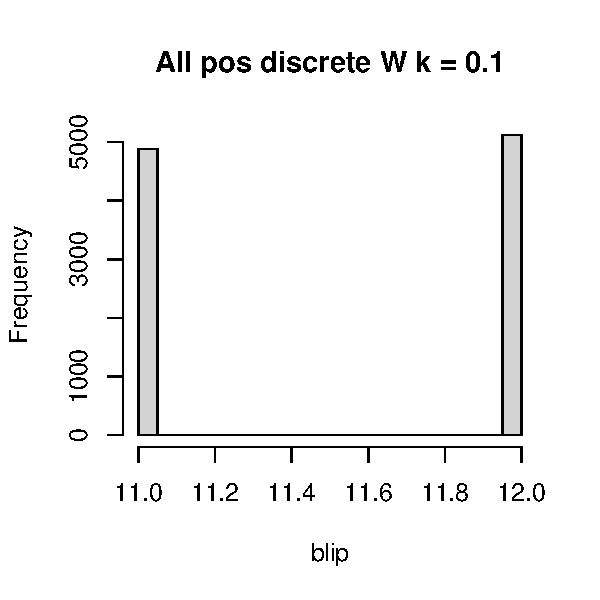
\includegraphics[width=\maxwidth]{figure/unnamed-chunk-4-1} 

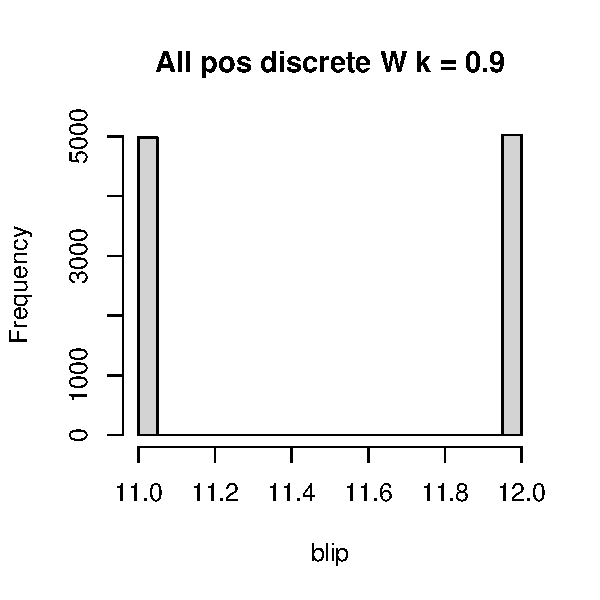
\includegraphics[width=\maxwidth]{figure/unnamed-chunk-4-2} 

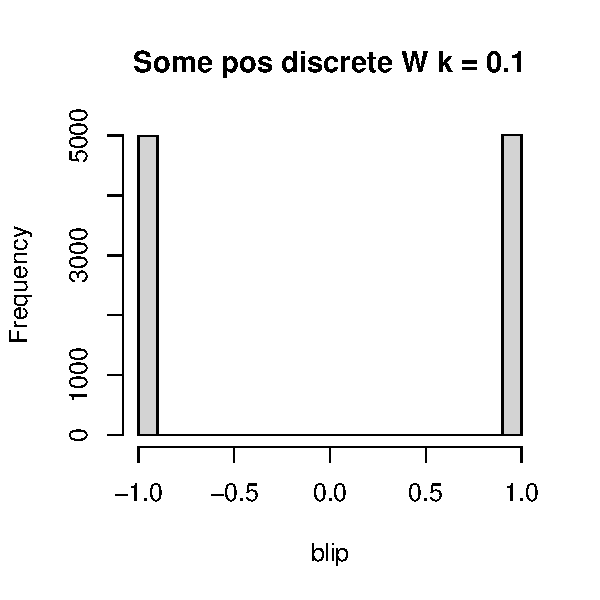
\includegraphics[width=\maxwidth]{figure/unnamed-chunk-4-3} 

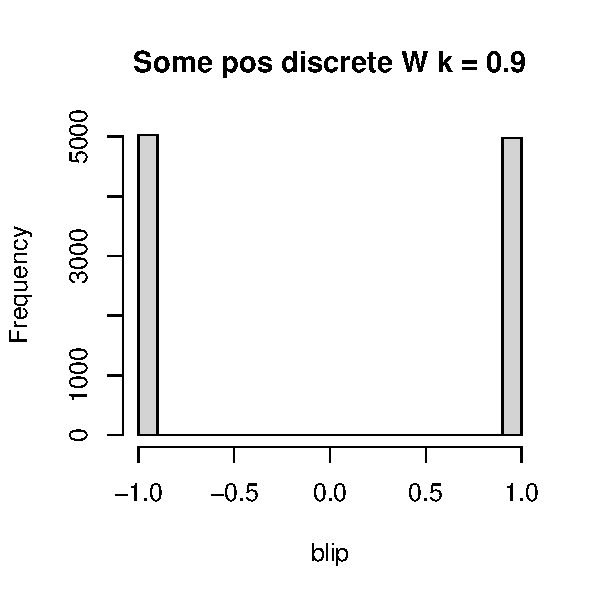
\includegraphics[width=\maxwidth]{figure/unnamed-chunk-4-4} 

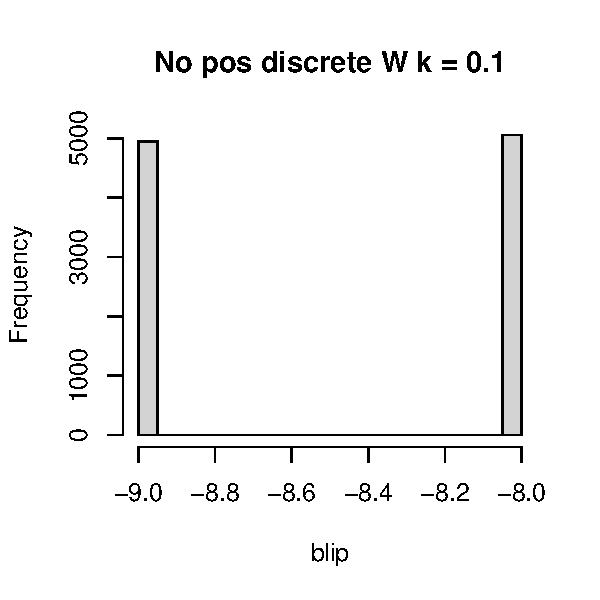
\includegraphics[width=\maxwidth]{figure/unnamed-chunk-4-5} 

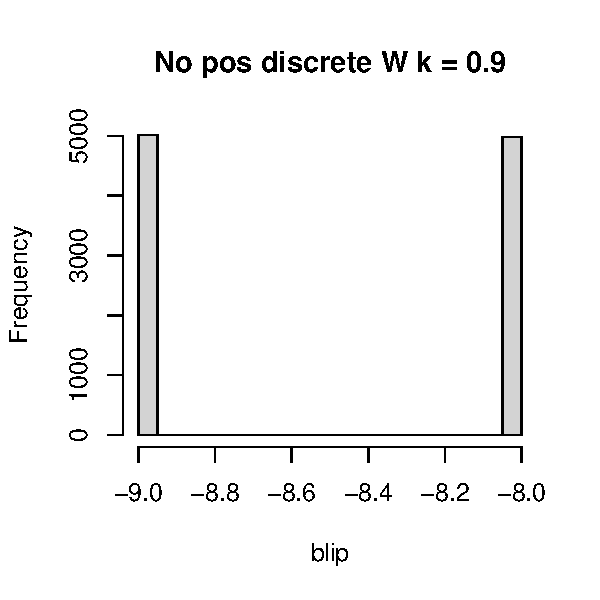
\includegraphics[width=\maxwidth]{figure/unnamed-chunk-4-6} 

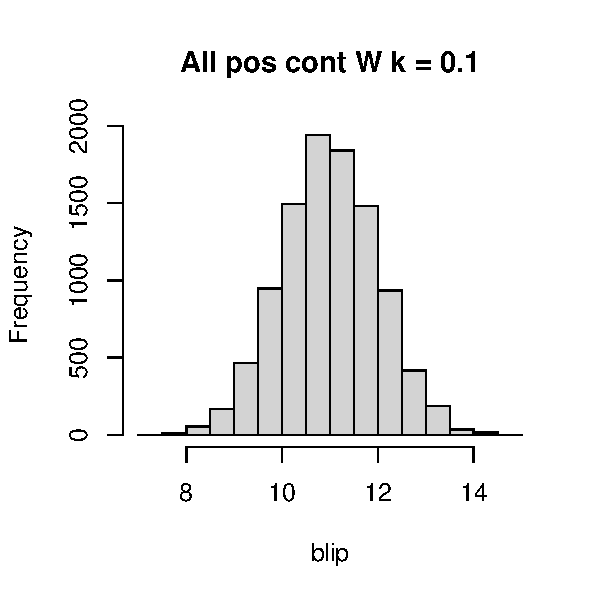
\includegraphics[width=\maxwidth]{figure/unnamed-chunk-4-7} 

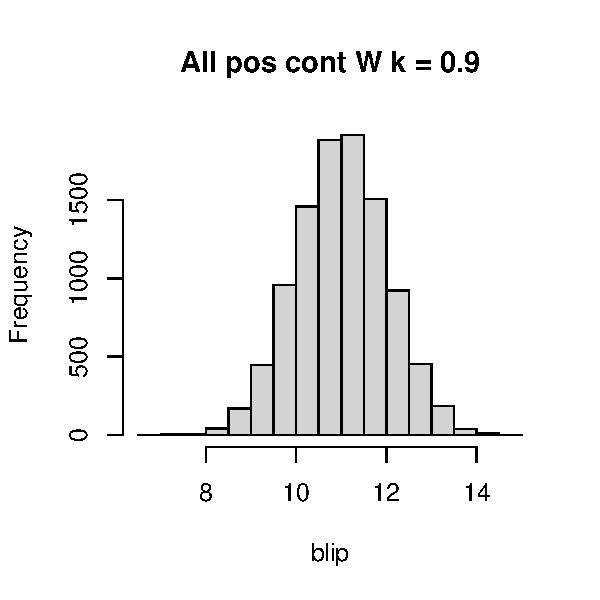
\includegraphics[width=\maxwidth]{figure/unnamed-chunk-4-8} 

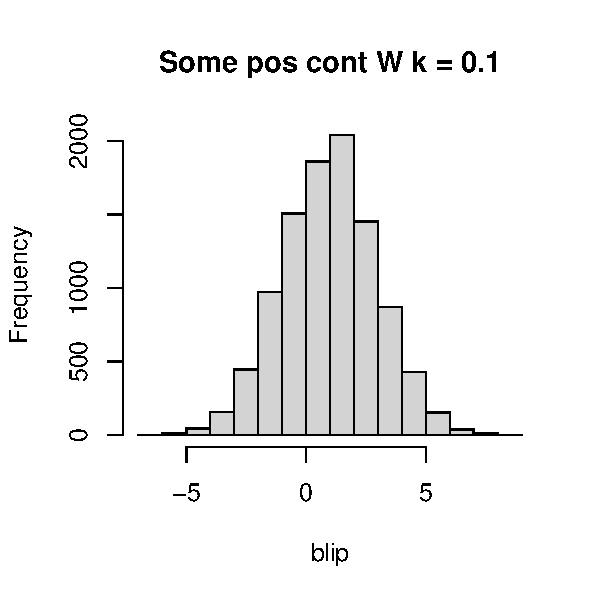
\includegraphics[width=\maxwidth]{figure/unnamed-chunk-4-9} 

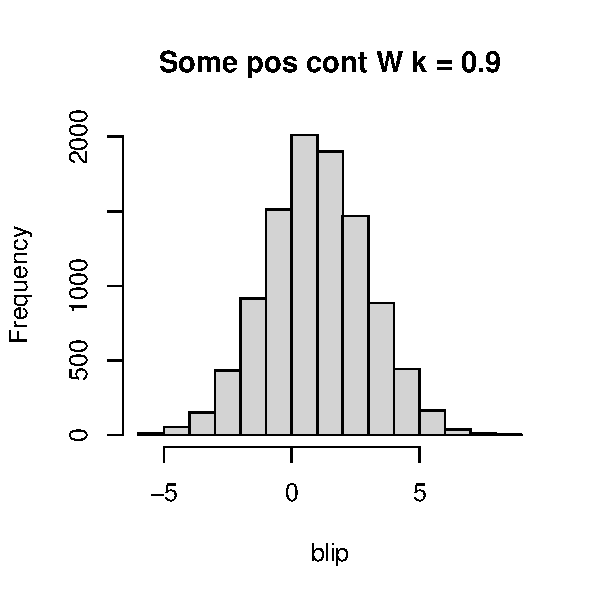
\includegraphics[width=\maxwidth]{figure/unnamed-chunk-4-10} 

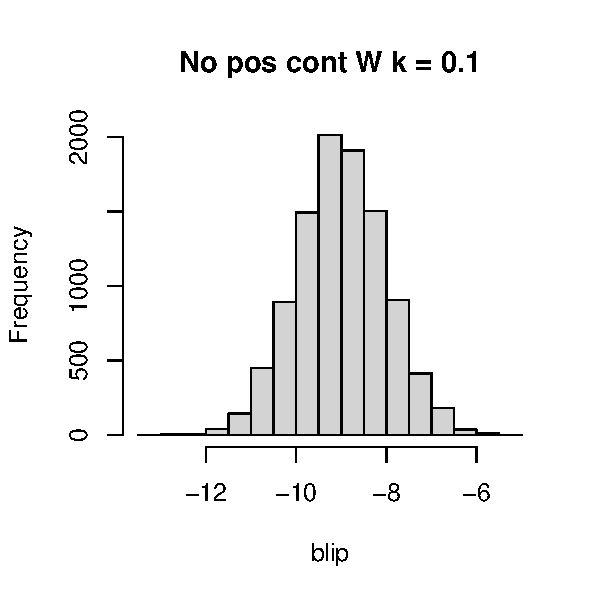
\includegraphics[width=\maxwidth]{figure/unnamed-chunk-4-11} 

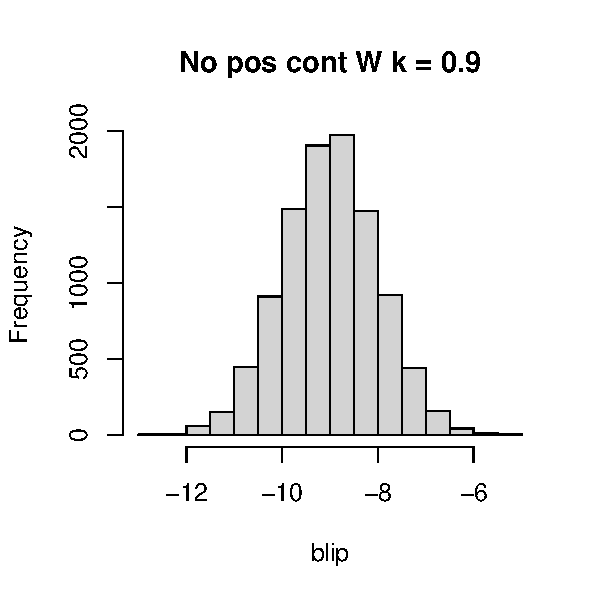
\includegraphics[width=\maxwidth]{figure/unnamed-chunk-4-12} 

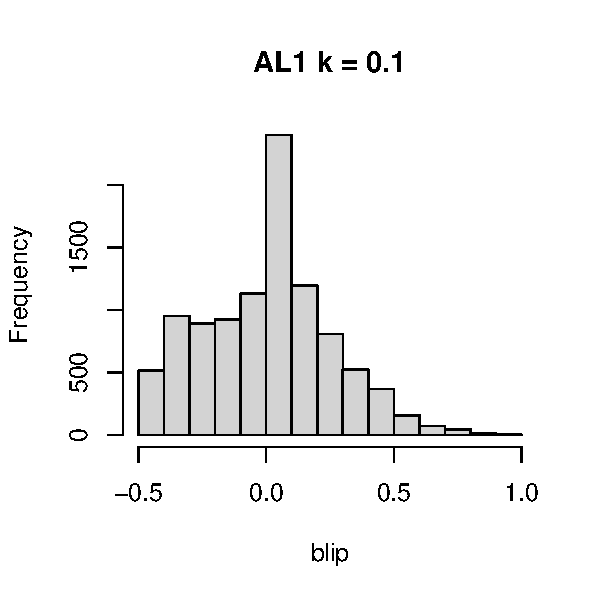
\includegraphics[width=\maxwidth]{figure/unnamed-chunk-4-13} 

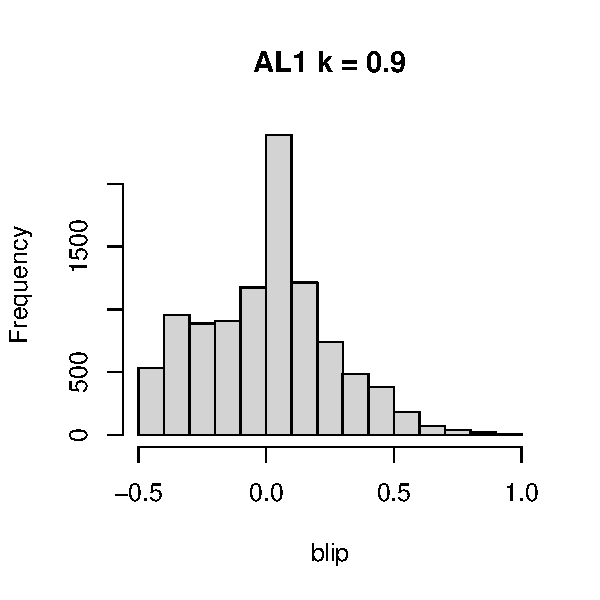
\includegraphics[width=\maxwidth]{figure/unnamed-chunk-4-14} 

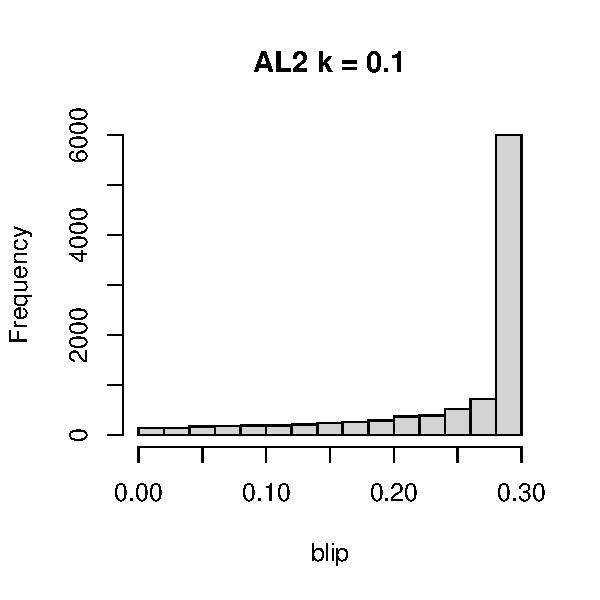
\includegraphics[width=\maxwidth]{figure/unnamed-chunk-4-15} 

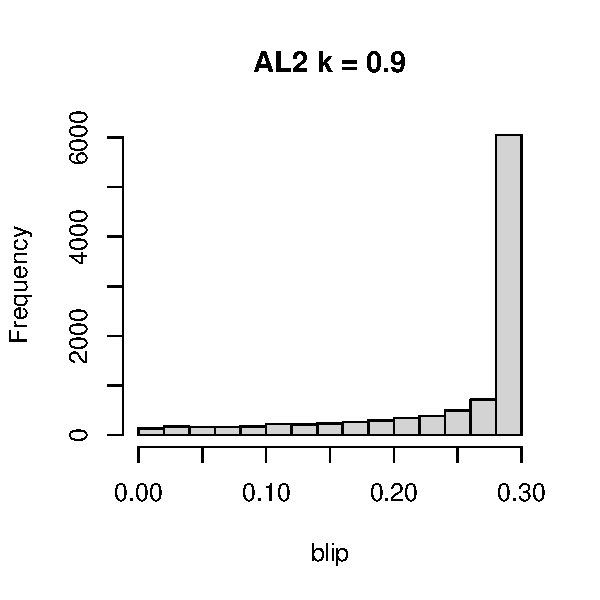
\includegraphics[width=\maxwidth]{figure/unnamed-chunk-4-16} 
\end{knitrout}







\end{document}
